
\newpage

\subsection{Пример использования}


Для демонстрации работы приложения был создан небольшой бот, который
просит ввести пользователя его имя и после выводит приветствие с использованием
данного имени.
Экранные формы примера работы приложения представлены на рисунках~
\ref{f:example:editor}-\ref{f:example:telegram}.

\begin{figure}[ht]
	\centering
	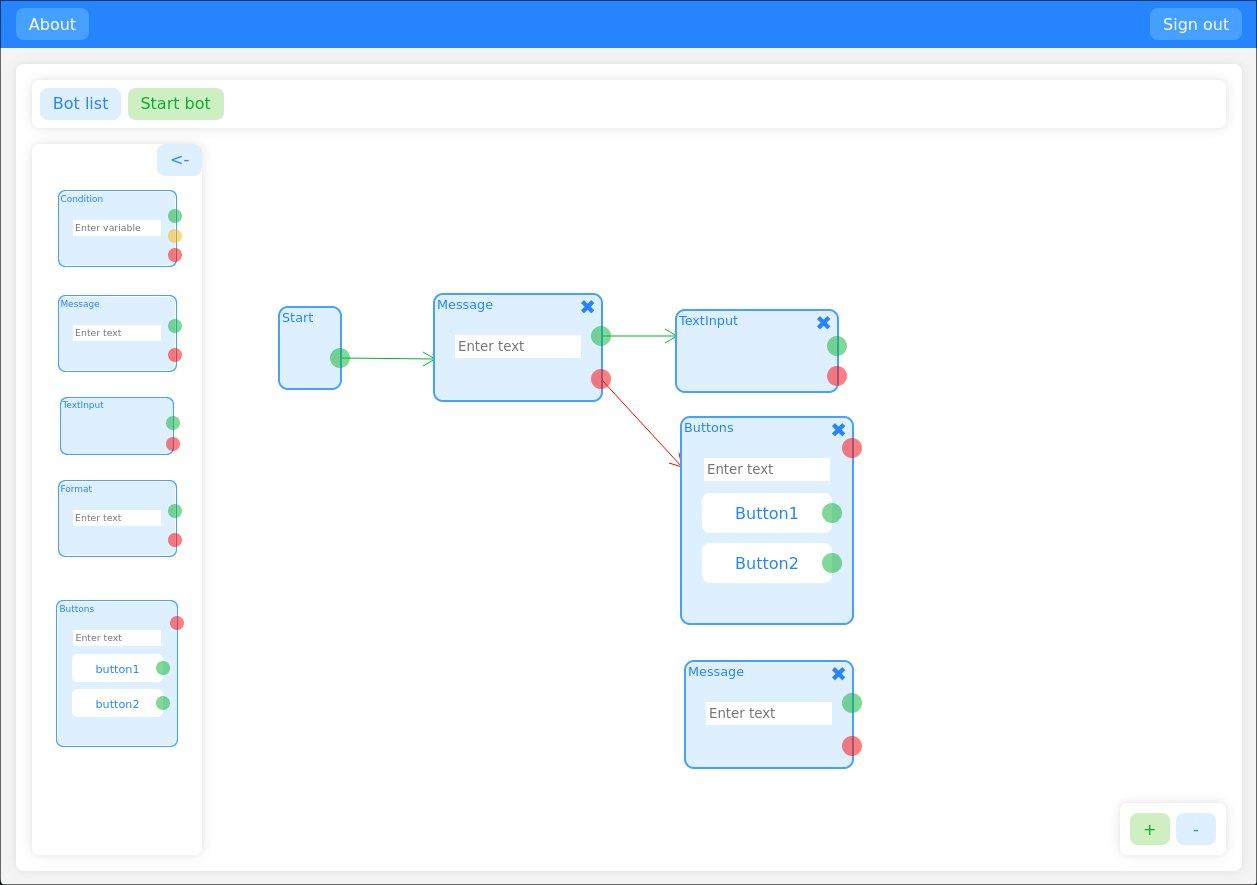
\includegraphics[width=\textwidth]{/example/editor}
	\caption{Построение структуры бота}
	\label{f:example:editor}
\end{figure}

\begin{figure}[ht]
	\centering
	
\includegraphics[width=0.9\textwidth]{/example/telegram}
	\caption{Использование созданного бота}
	\label{f:example:telegram}
\end{figure}


